\chapter{Calorimeter Optimisation Studies}
\label{chap:MoreStuff}

\chapterquote{There, sir! that is the perfection of vessels!}
{Jules Verne, 1828--1905}

\section{Calorimeter Optimisation Studies}


% \begin{figure}
%   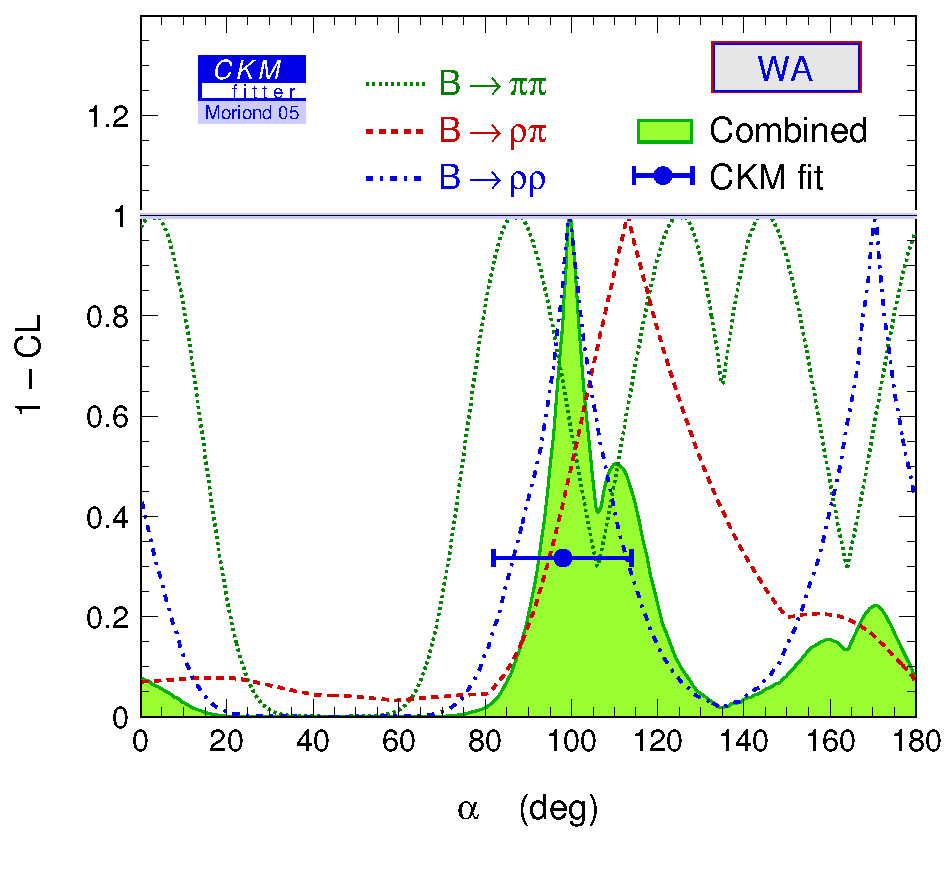
\includegraphics[width=\largefigwidth]{ckmfitter-alpha-combined}
%   \caption[CKM Fitter constraints on \alphaCKM.]%
%   {CKM Fitter constraints on \alphaCKM from combined \BToPiPi,
%     \BToRhoPi and \BToRhoRho decay analyses.}
%   \label{fig:CKMFitter}
% \end{figure}

\section{Electromagnetic Calorimeter Optimisation}
\label{optstud:sec:ecal}

\subsection{ECal Transverse Granularity}
\label{optstud:sec:ecal:cellsize}

\begin{figure}
  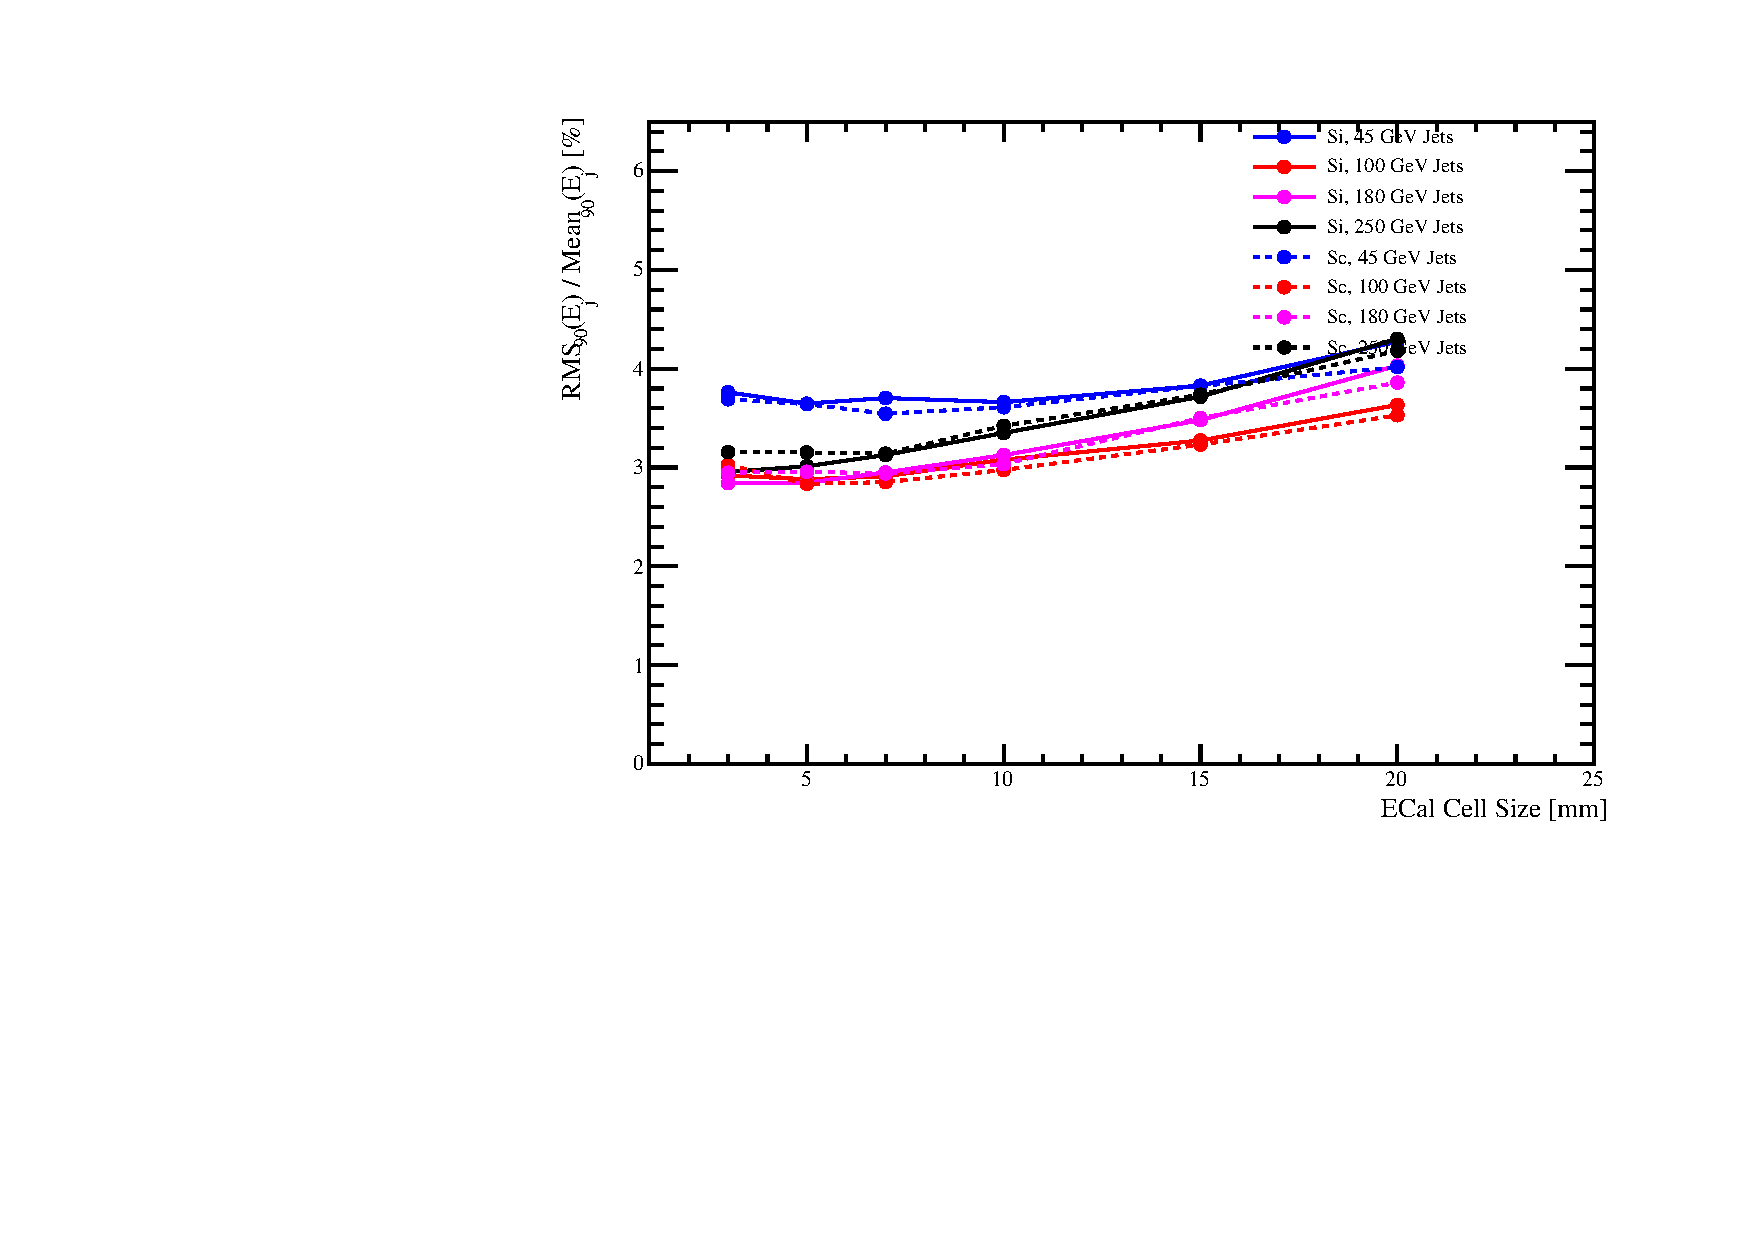
\includegraphics[width=\largefigwidth]{OptimisationStudies/Plots/JER_vs_SiliconECalCellSize.pdf}
  \caption[Jet energy resolution as a function of ECal cell size for the silicon tungsten ECal option.]{Jet energy resolution is shown for several fixed energy jets as a function of ECal cell size for the silicon tungsten ECal option.}
  \label{optstud:fig:siecalcells}
\end{figure}

\begin{figure}
  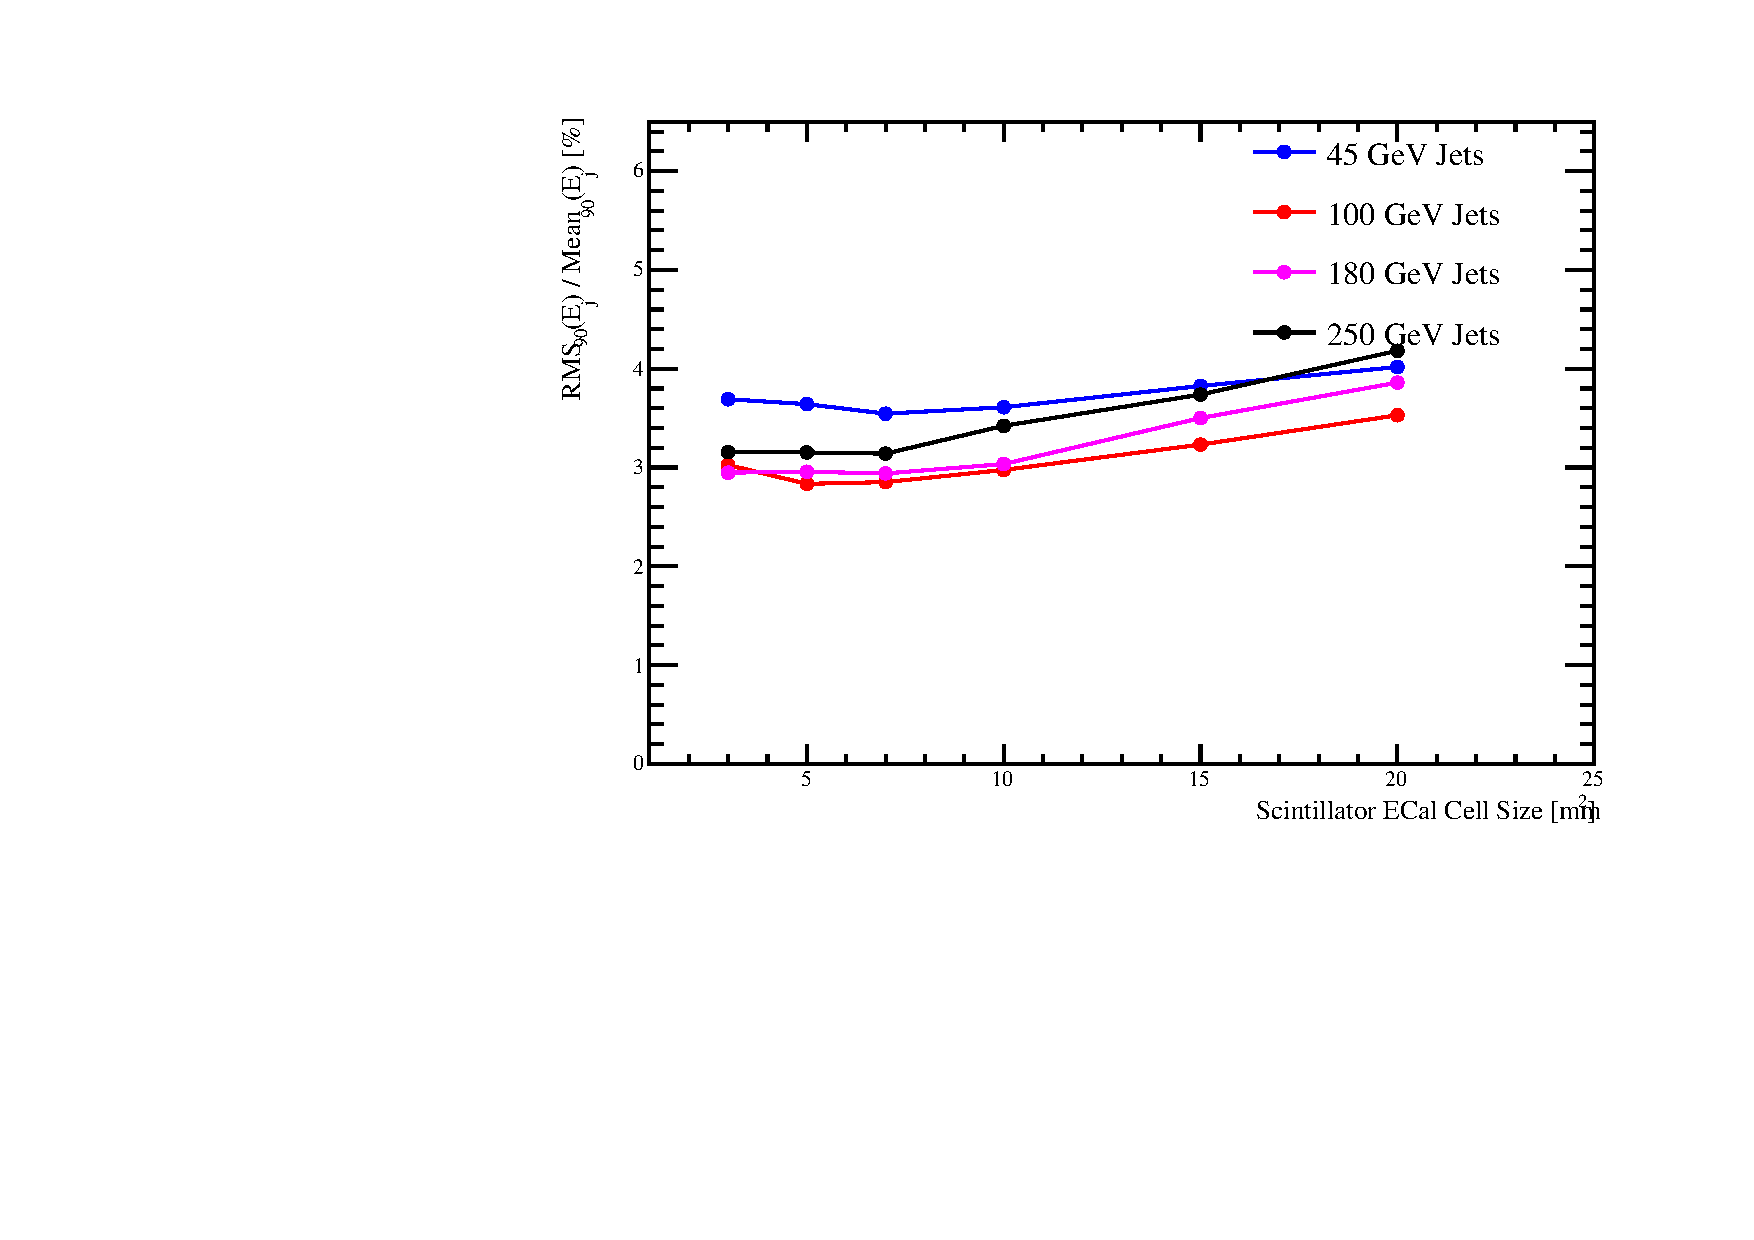
\includegraphics[width=\largefigwidth]{OptimisationStudies/Plots/JER_vs_ScintillatorECalCellSize.pdf}
  \caption[Jet energy resolution as a function of ECal cell size for the scintillator tungsten ECal option.]{Jet energy resolution is shown for several fixed energy jets as a function of ECal cell size for the scintillator tungsten ECal option.}
  \label{optstud:fig:scecalcells}
\end{figure}

\subsection{ECal Longitudinal Granularity}
\label{optstud:sec:ecal:nlayers}

\begin{figure}
  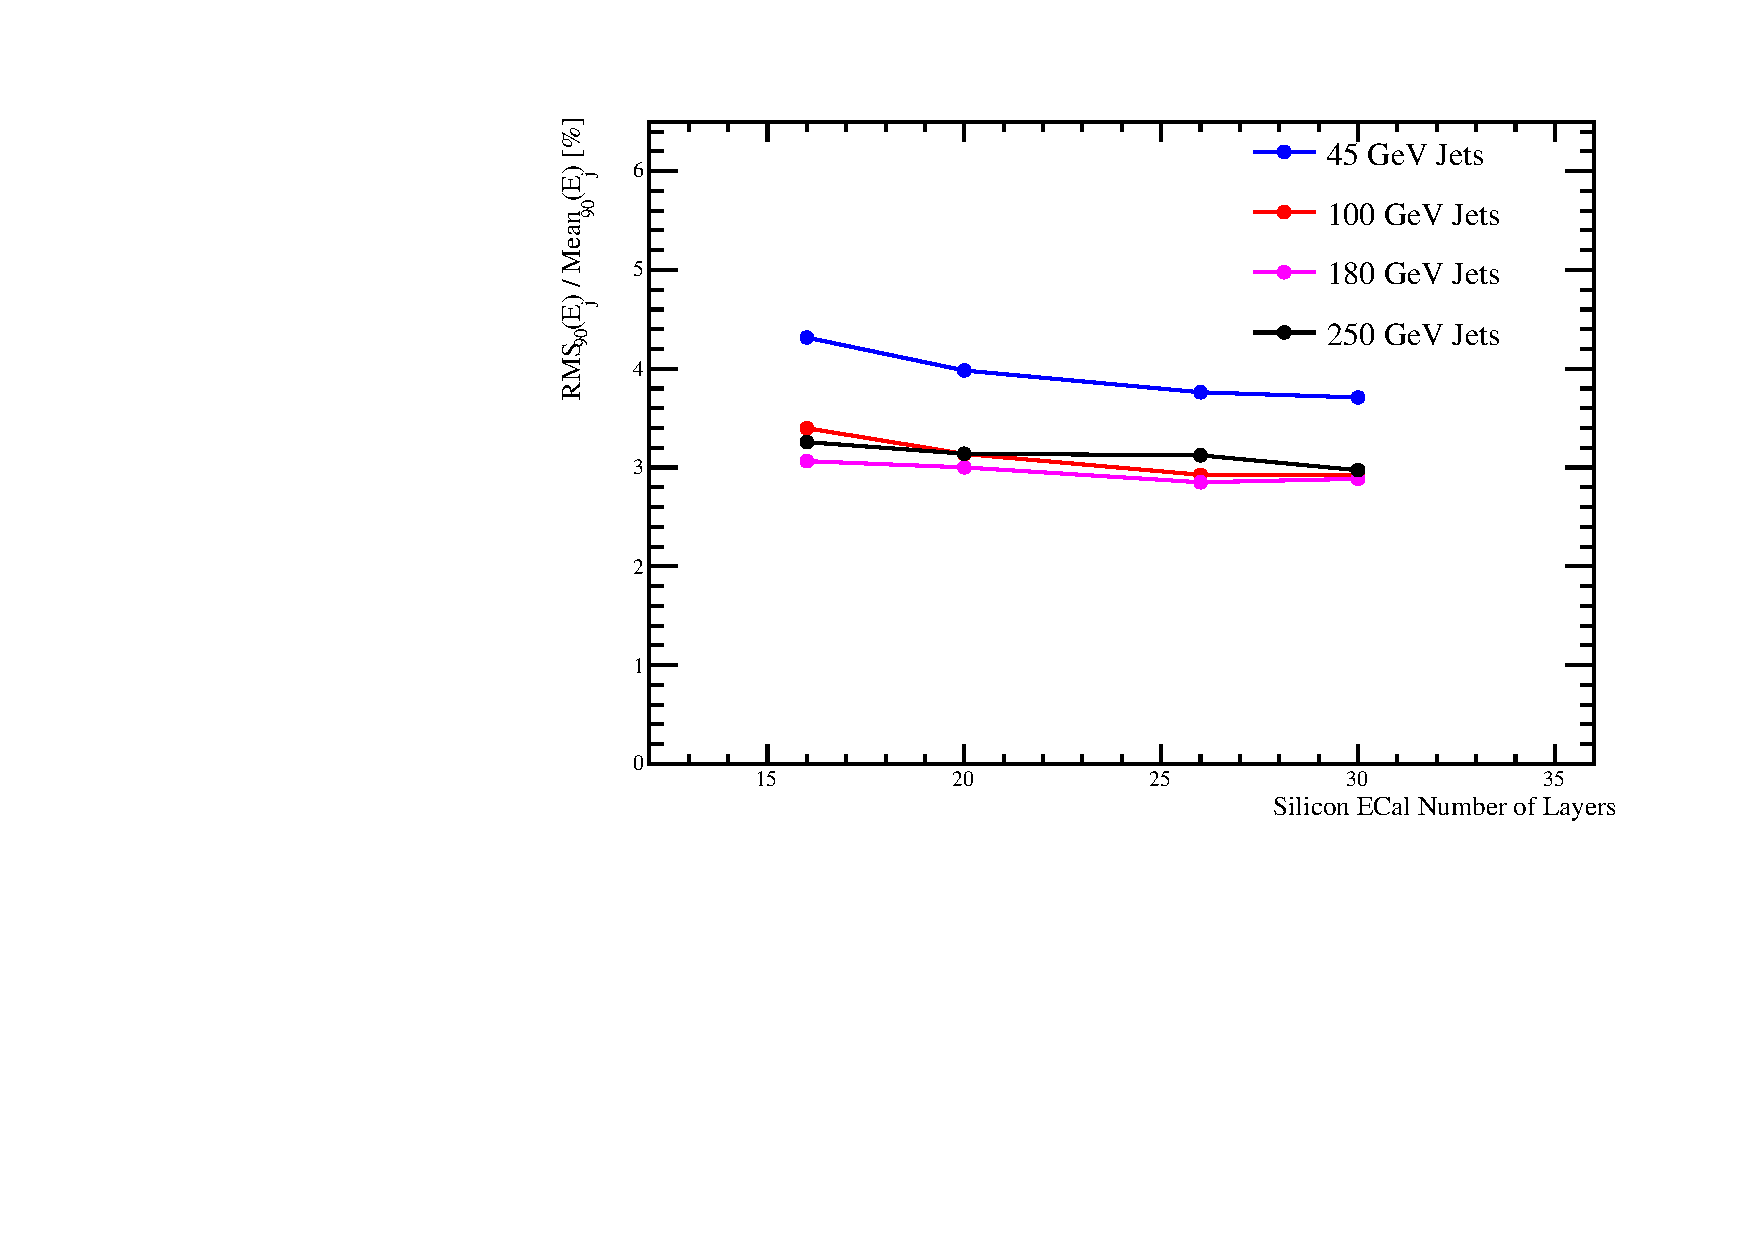
\includegraphics[width=\largefigwidth]{OptimisationStudies/Plots/JER_vs_SiliconECalNumberofLayers.pdf}
  \caption[Jet energy resolution as a function of the number of layers in the ECal for the silicon tungsten ECal option.]{Jet energy resolution is shown for several fixed energy jets as a function of the number of layers in the ECal for the silicon tungsten ECal option.}
  \label{optstud:fig:siecallayers}
\end{figure}

\begin{figure}
  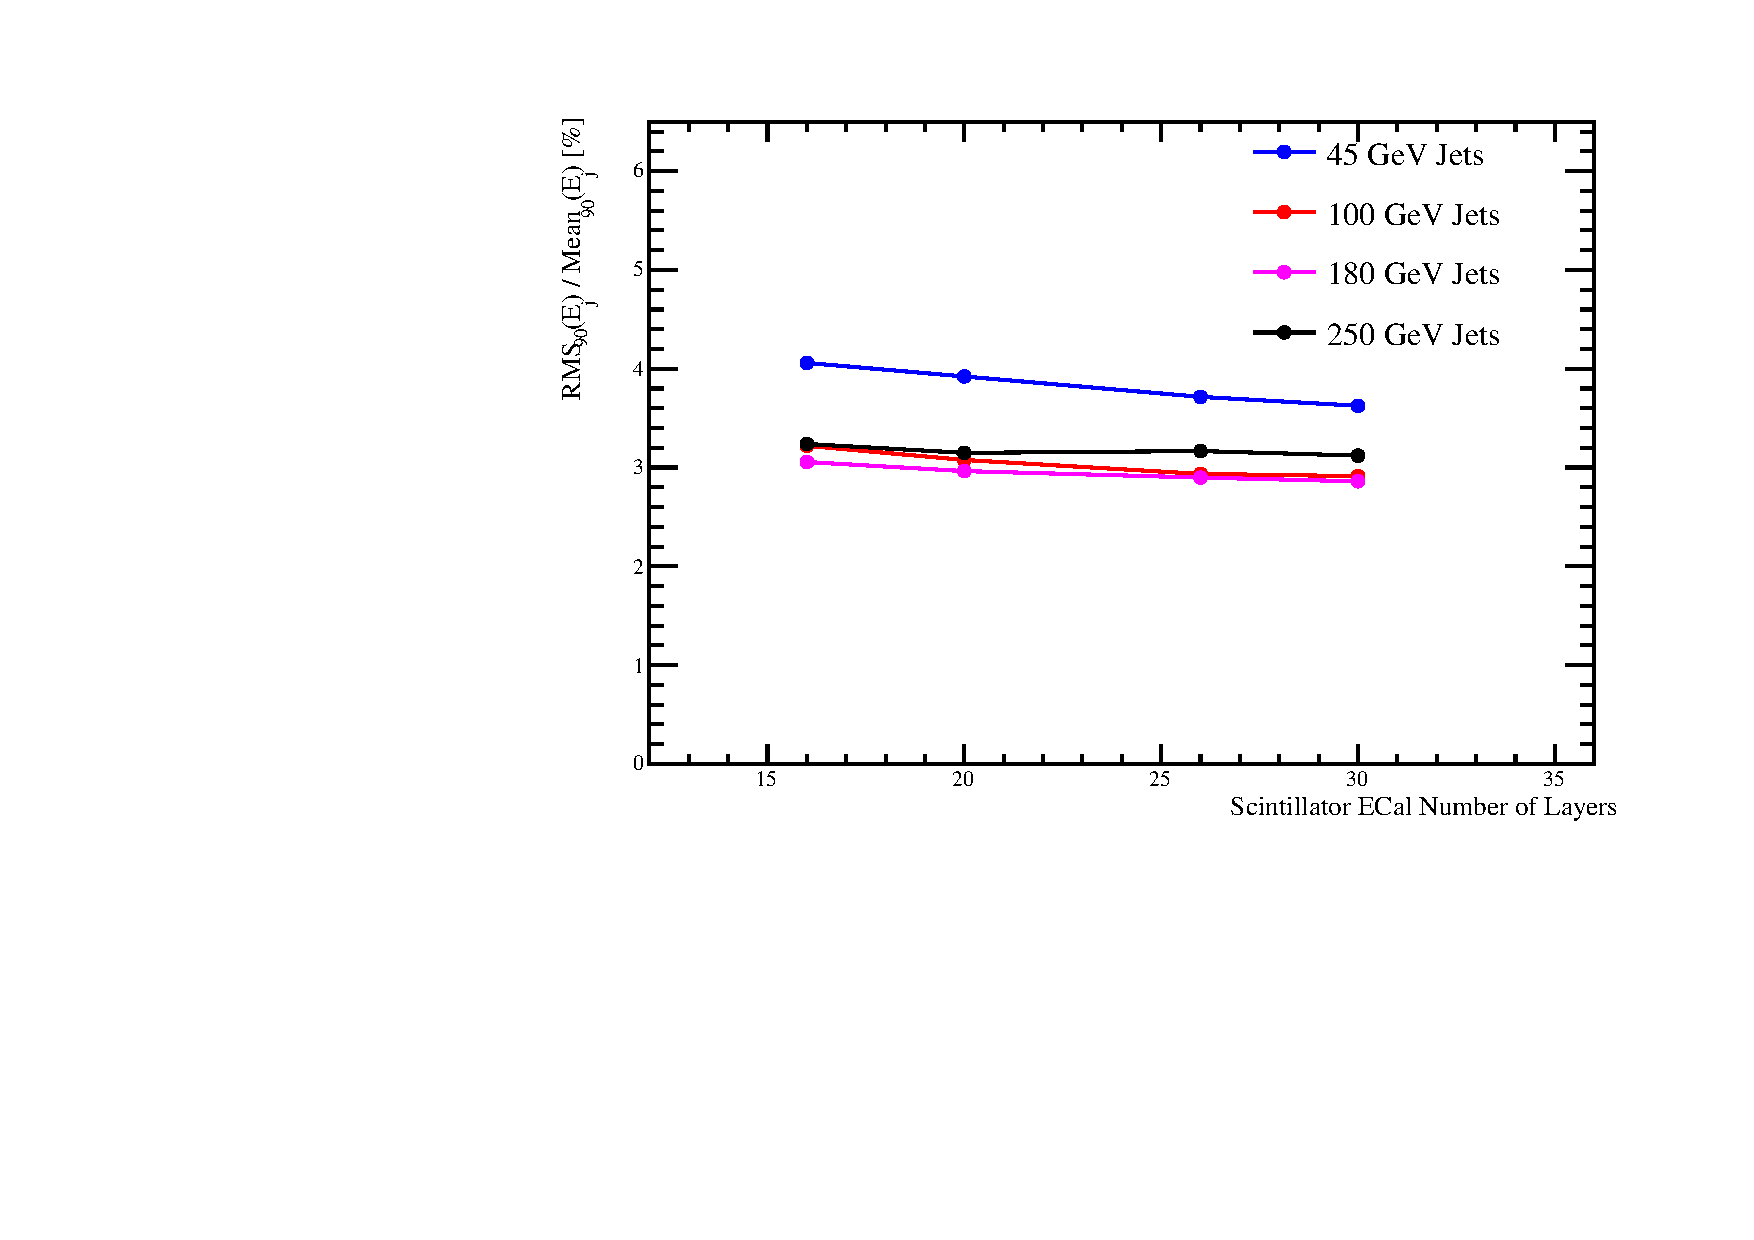
\includegraphics[width=\largefigwidth]{OptimisationStudies/Plots/JER_vs_ScintillatorECalNumberofLayers.pdf}
  \caption[Jet energy resolution as a function of the number of layers in the ECal for the scintillator tungsten ECal option.]{Jet energy resolution is shown for several fixed energy jets as a function of the number of layers in the ECal for the scintillator tungsten ECal option.}
  \label{optstud:fig:scecallayers}
\end{figure}

\section{Hadronic Calorimeter Optimsation}
\label{optstud:sec:hcal}

\subsection{HCal Transverse Granularity}
\label{optstud:sec:hcal:cellsize}

\begin{figure}
  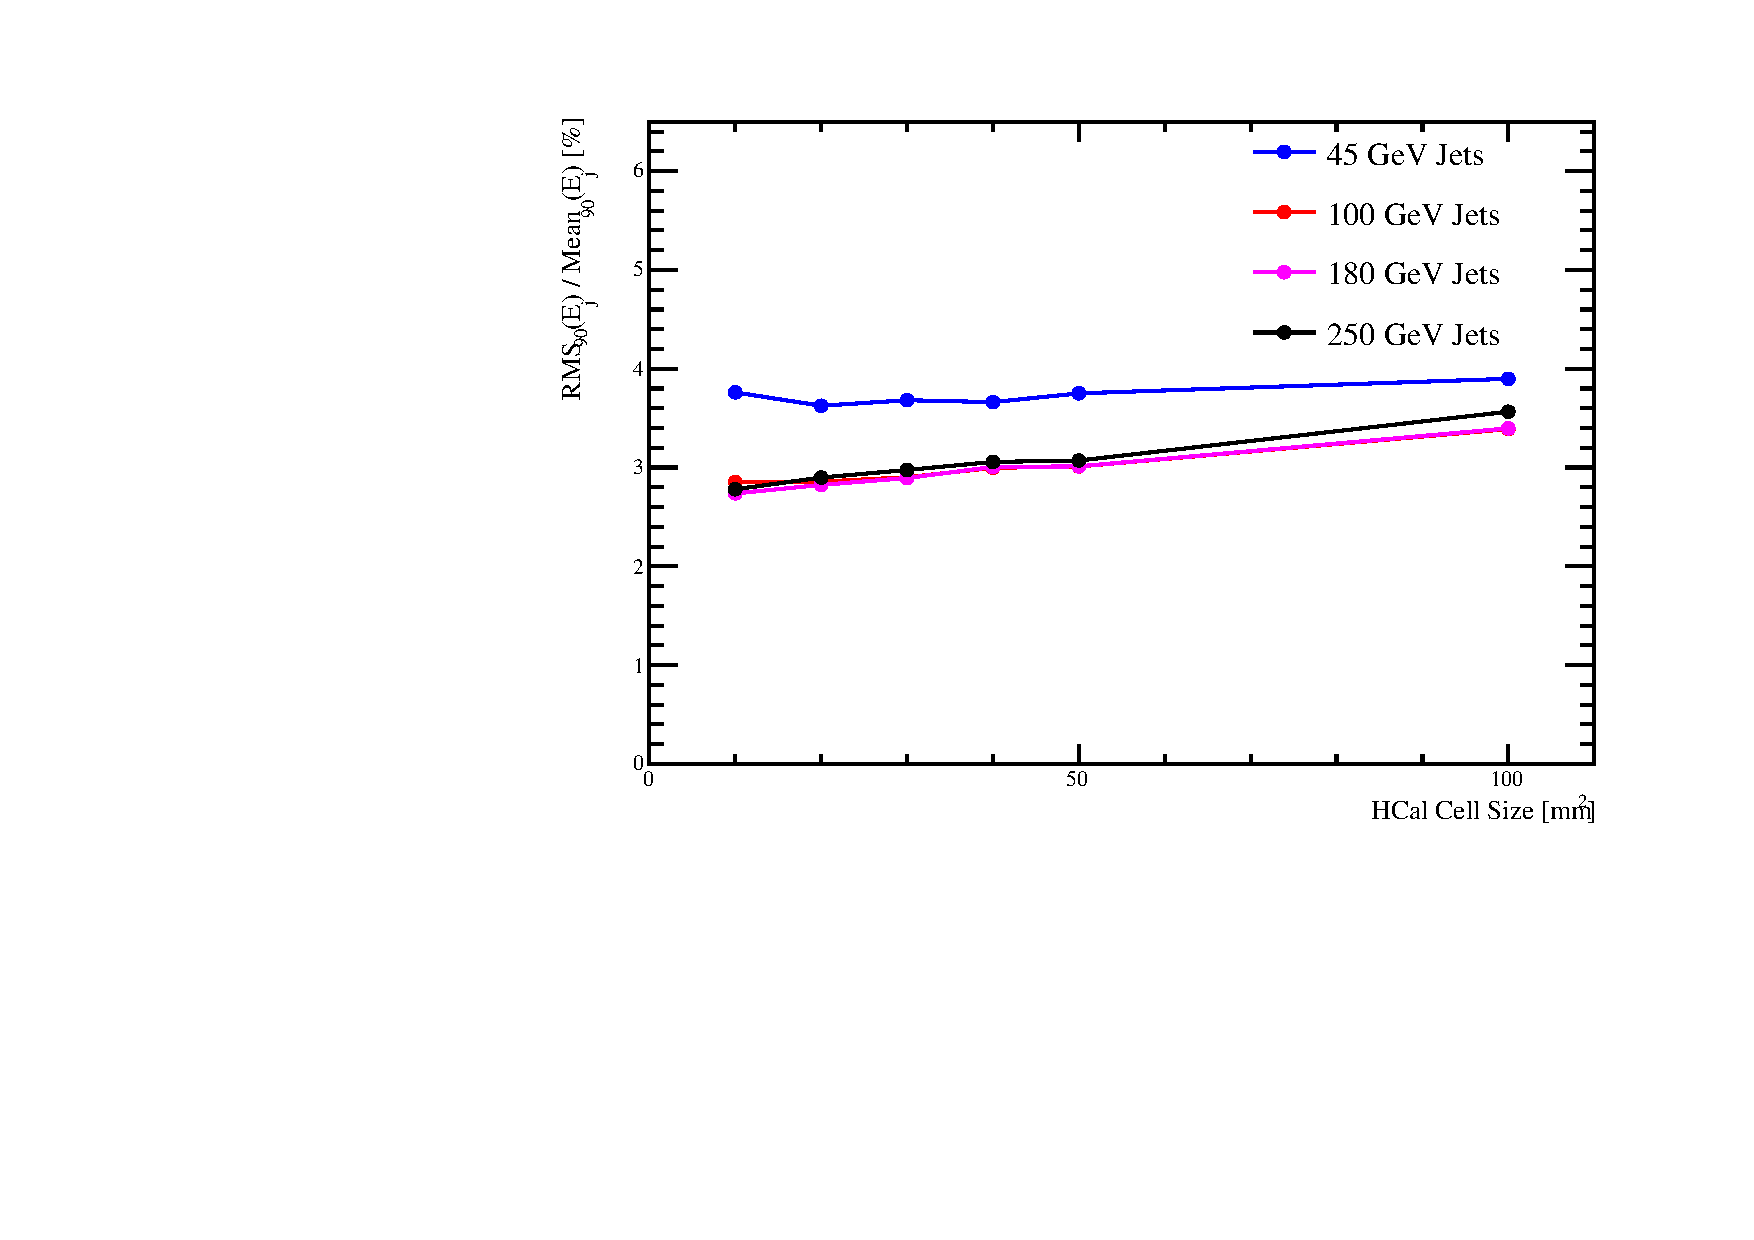
\includegraphics[width=\largefigwidth]{OptimisationStudies/Plots/JER_vs_HCalCellSize.pdf}
  \caption[Jet energy resolution as a function of HCal cell size for the scintillator steel HCal option.]{Jet energy resolution is shown for several fixed energy jets as a function of HCal cell size for the scintillator steel HCal option.}
  \label{optstud:fig:hcalcells}
\end{figure}

\subsection{HCal Longitudinal Granularity}
\label{optstud:sec:hcal:nlayers}

\begin{figure}
  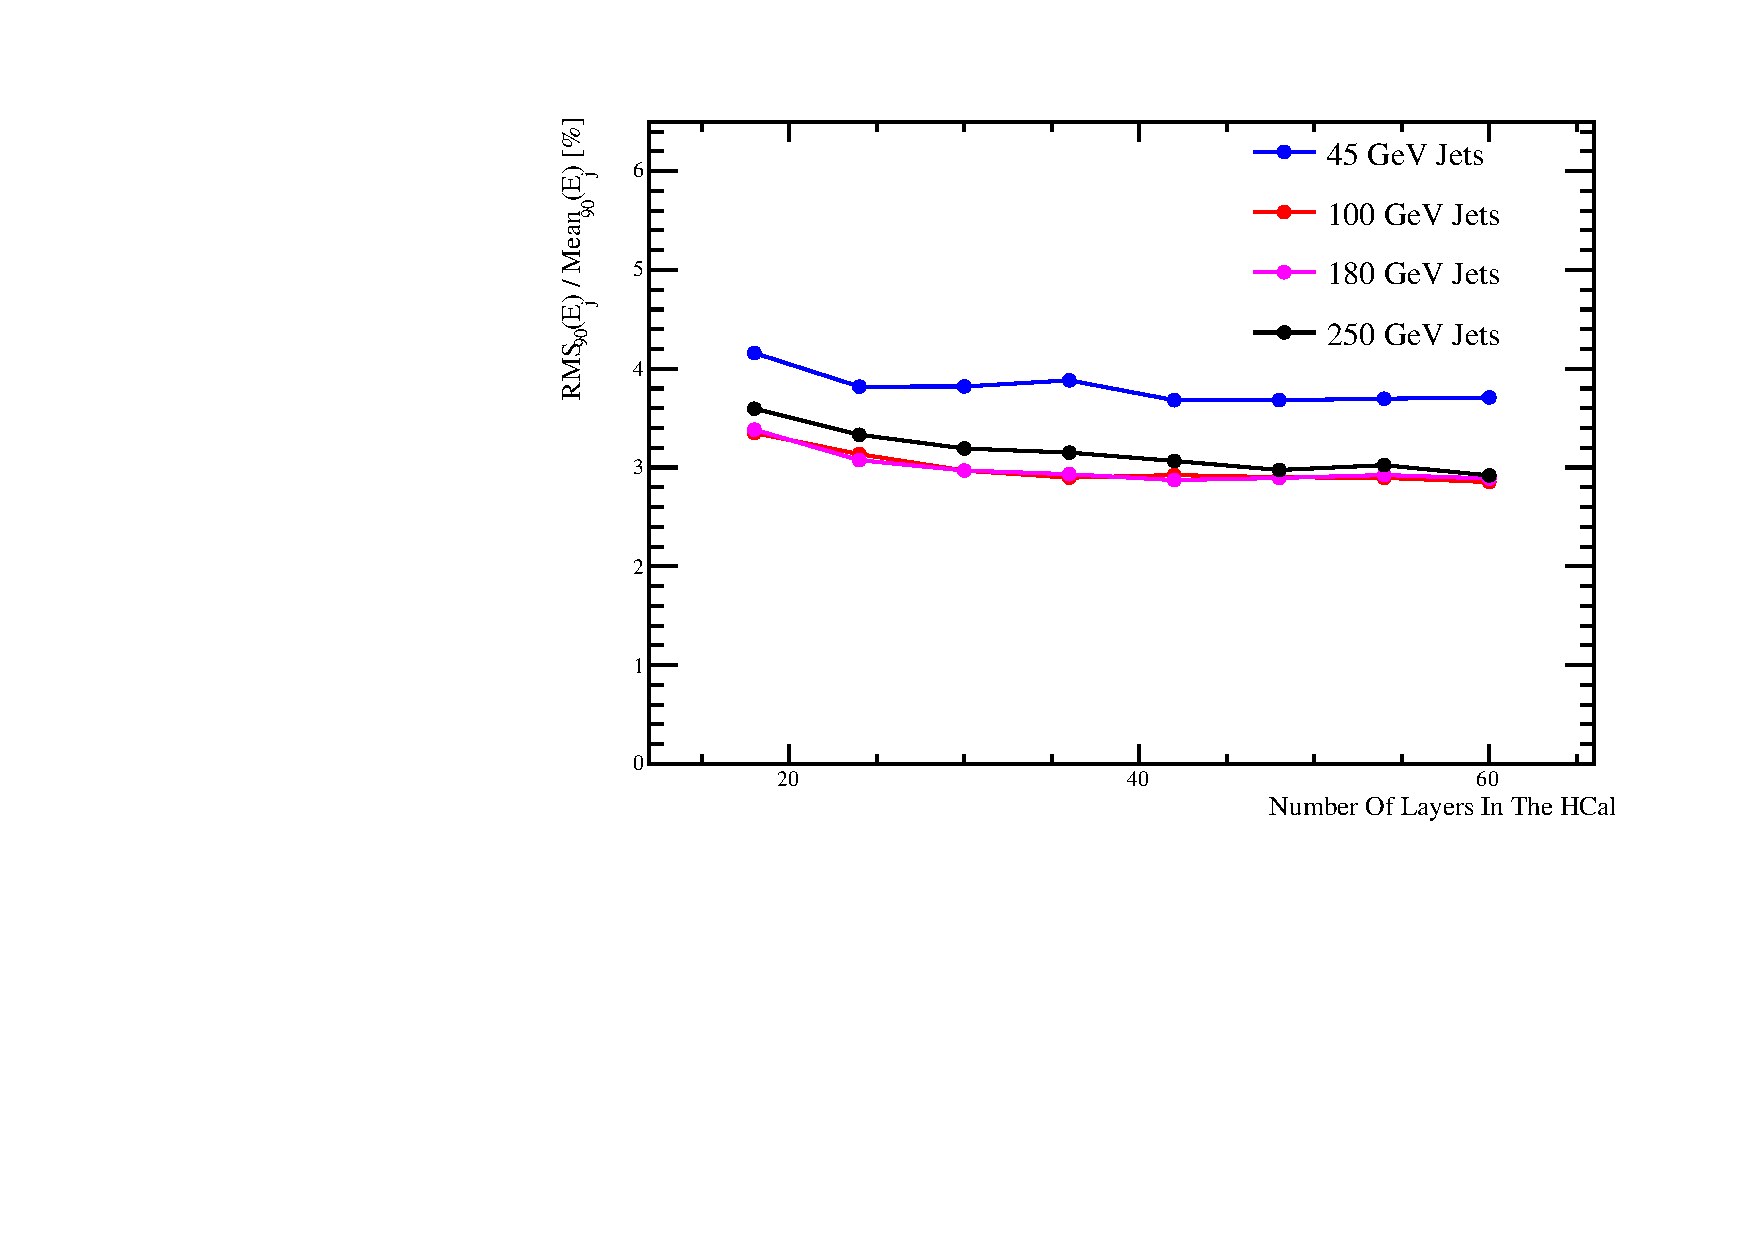
\includegraphics[width=\largefigwidth]{OptimisationStudies/Plots/JER_vs_NumberOfLayersInTheHCal.pdf}
  \caption[Jet energy resolution as a function of the number of layers in the HCal for the scintillator steel HCal option.]{Jet energy resolution is shown for several fixed energy jets as a function of the number of layers in the HCal for the scintillator steel HCal option.}
  \label{optstud:fig:hcalnlayers}
\end{figure}

\begin{figure}
  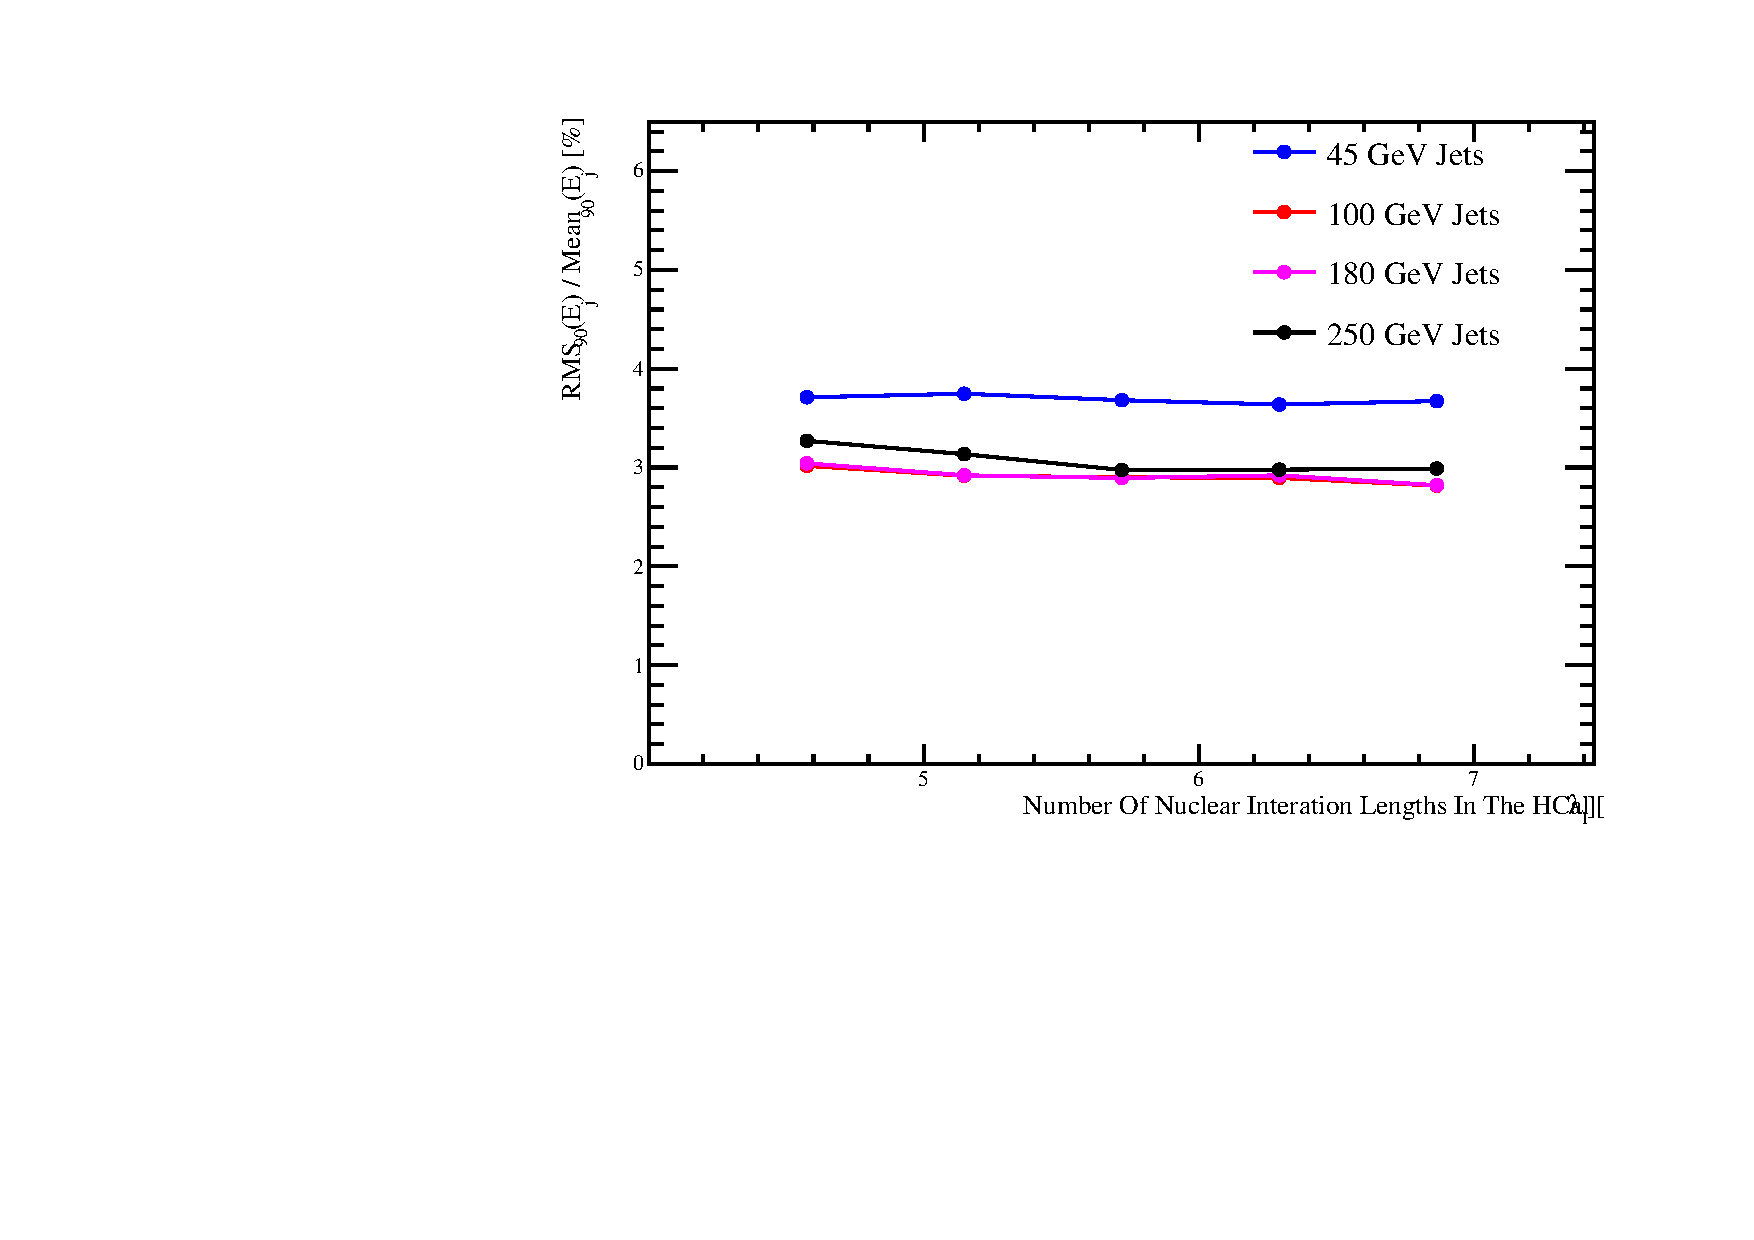
\includegraphics[width=\largefigwidth]{OptimisationStudies/Plots/JER_vs_NumberOfNuclearInterationLengthsInTheHCal.pdf}
  \caption[Jet energy resolution as a function of the number of nuclear interaction lengths in the HCal for the scintillator steel HCal option.]{Jet energy resolution is shown for several fixed energy jets as a function of the number of nuclear interation lenghts in the HCal for the scintillator steel HCal option.}
  \label{optstud:fig:hcaldepth}
\end{figure}

\begin{figure}
  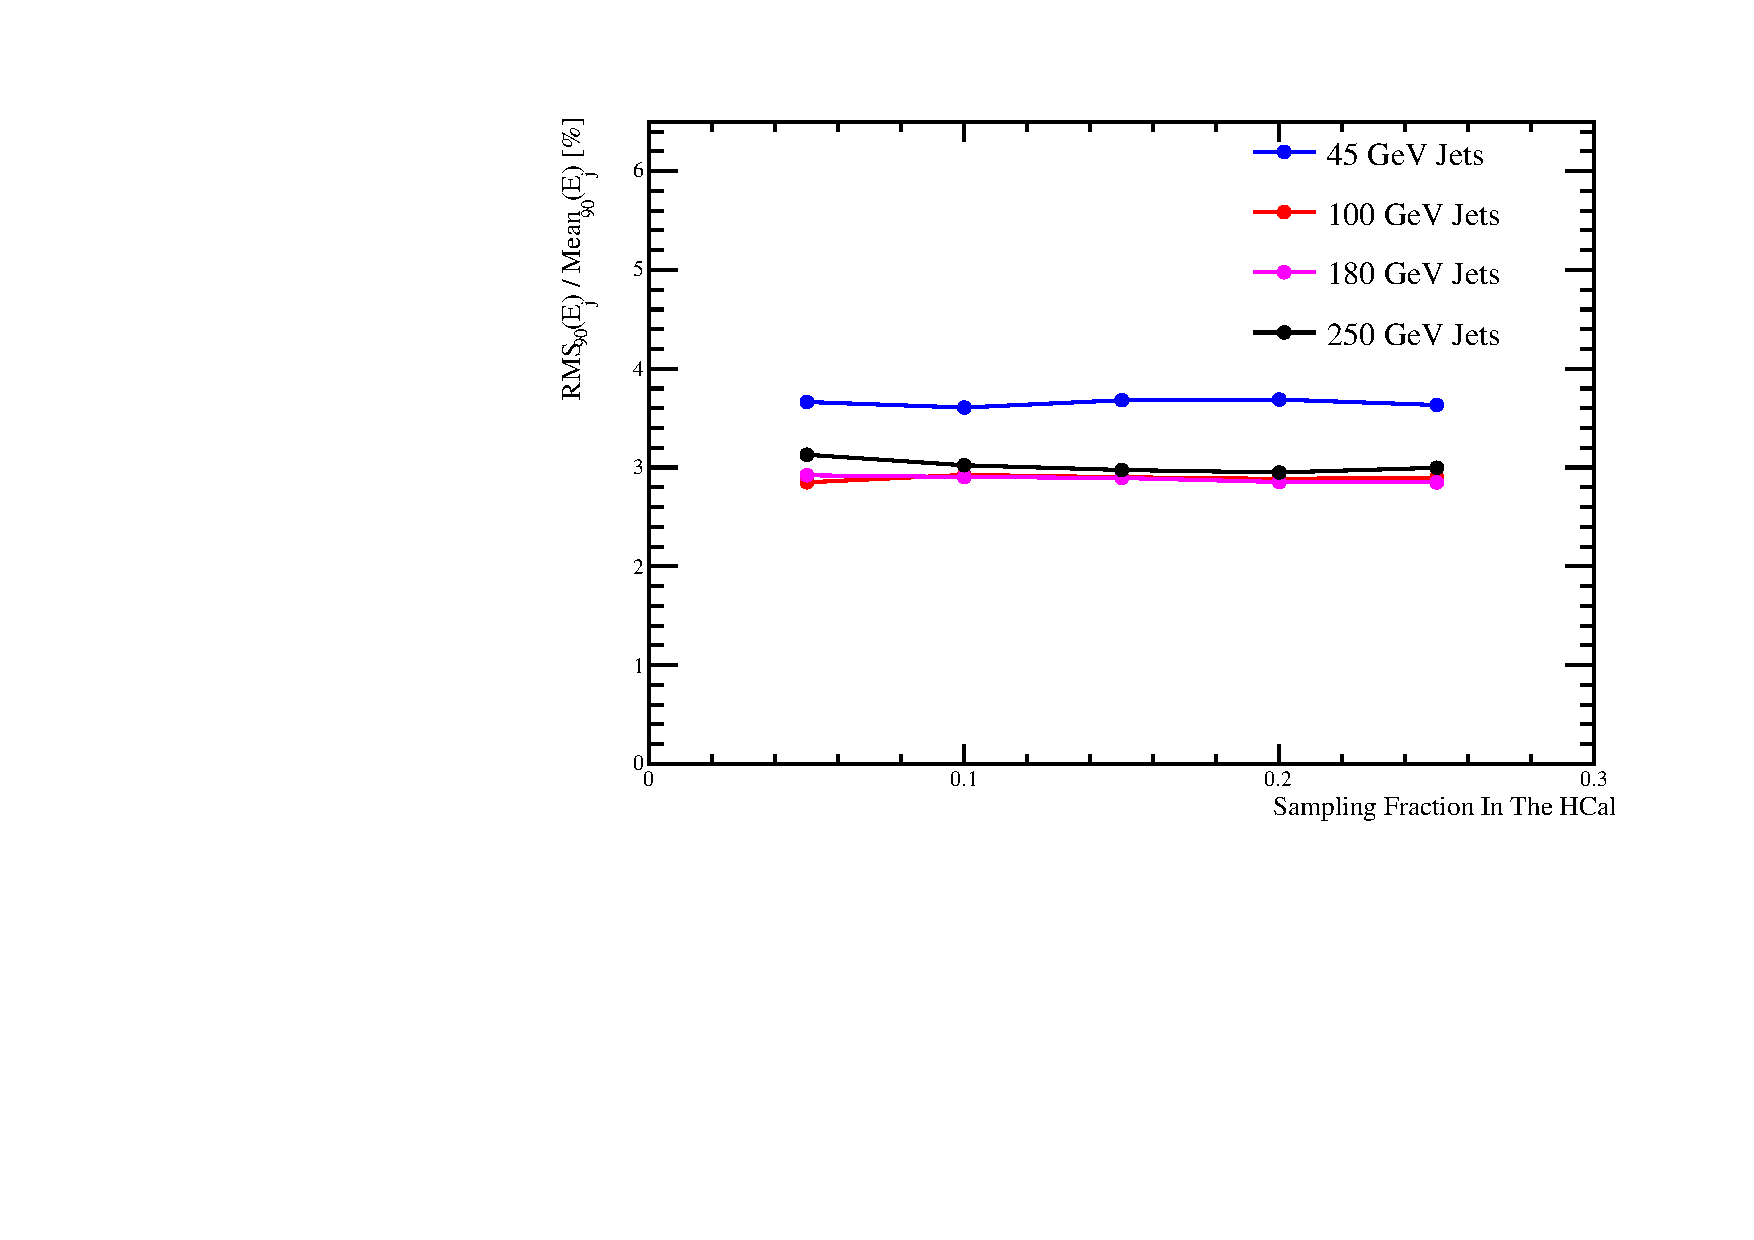
\includegraphics[width=\largefigwidth]{OptimisationStudies/Plots/JER_vs_SamplingFractionInTheHCal.pdf}
  \caption[Jet energy resolution as a function of the sampling fraction in the HCal for the scintillator steel HCal option.]{Jet energy resolution is shown for several fixed energy jets as a function of the sampling fraction in the HCal for the scintillator steel HCal option.}
  \label{optstud:fig:hcalsampfrac}
\end{figure}

\subsection{HCal Absorber Material}
\label{optstud:sec:hcal:absmat}

\begin{figure}
  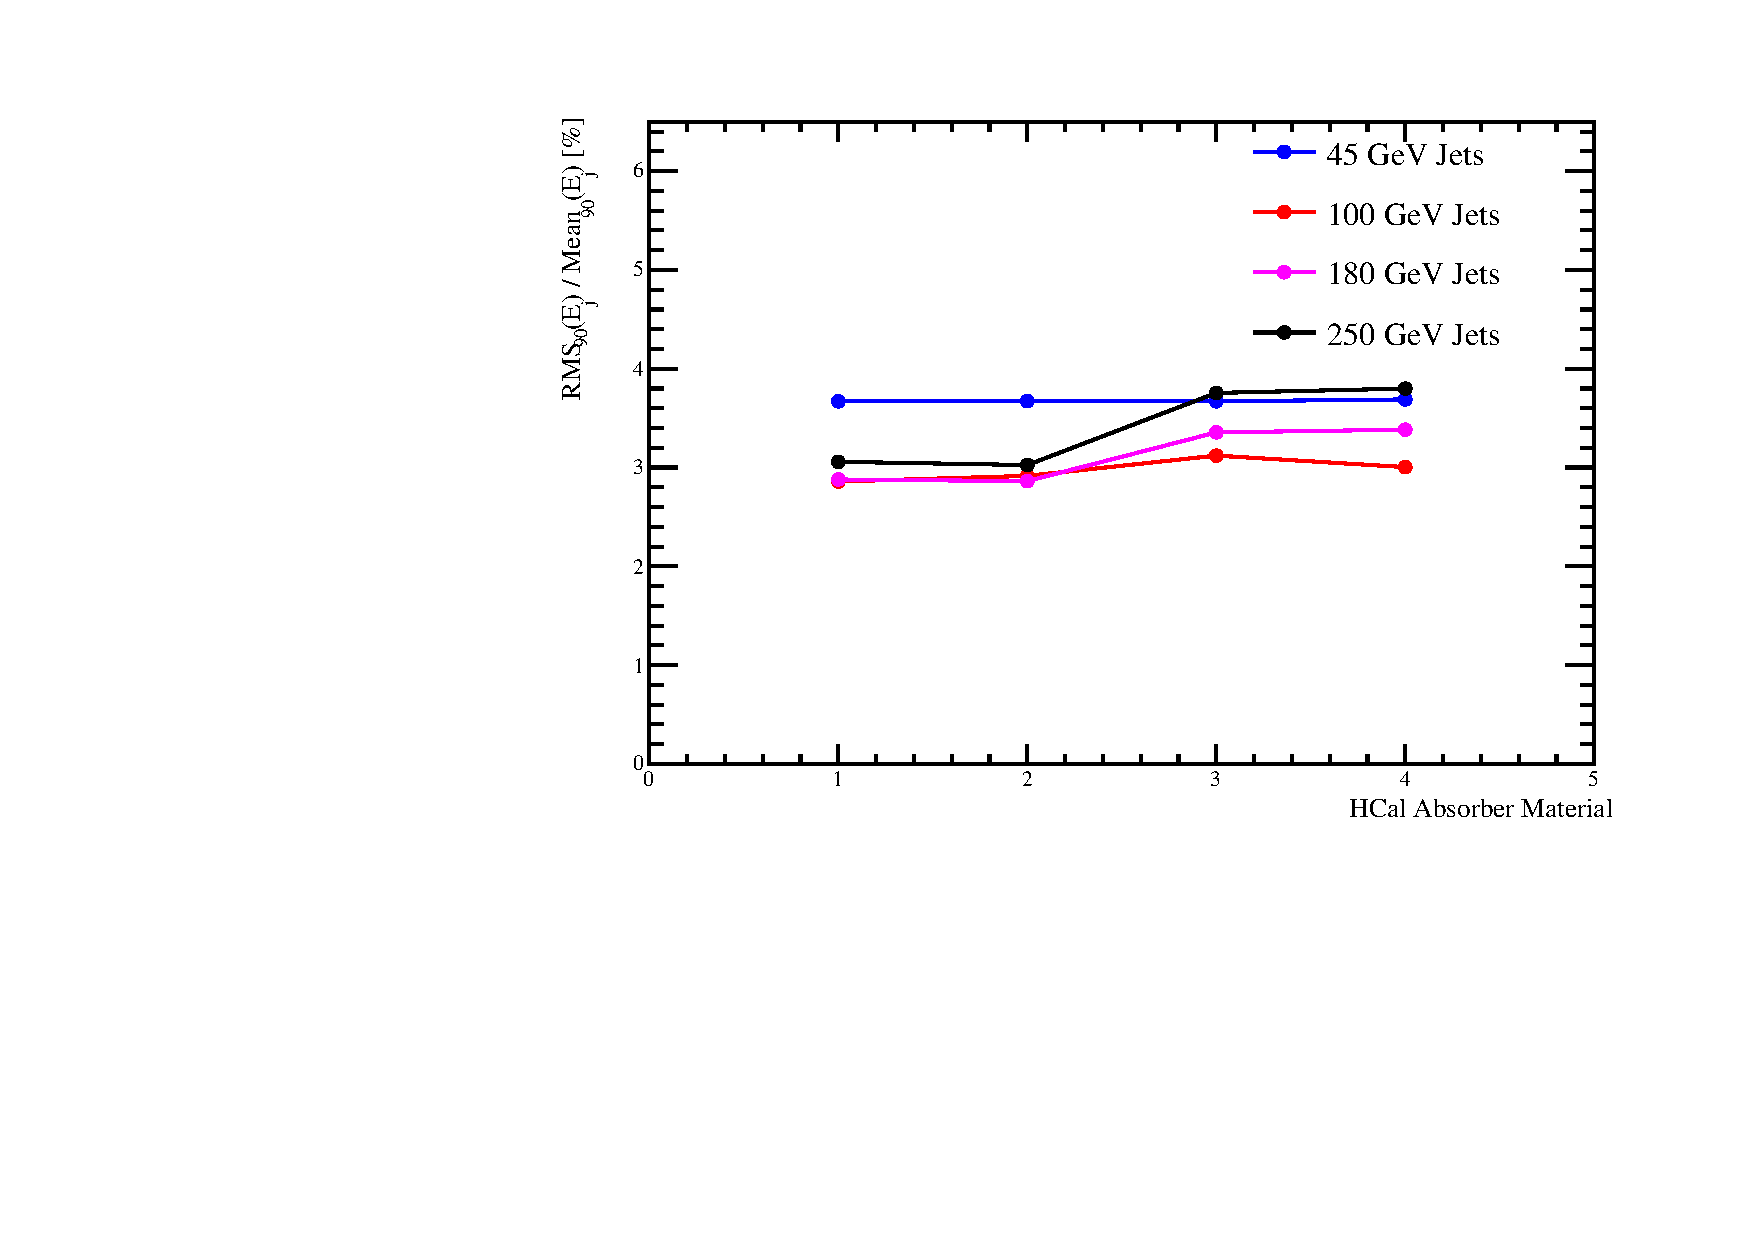
\includegraphics[width=\largefigwidth]{OptimisationStudies/Plots/JER_vs_HCalAbsorberMaterial.pdf}
  \caption[Jet energy resolution as a function of the absorber matieral in the HCal.]{Jet energy resolution is shown for several fixed energy jets as a function of the absorber material in the HCal.}
  \label{optstud:fig:hcalabsmat}
\end{figure}

\section{Global Detector Parameter Optimisation}
\label{optstud:sec:global}

\subsection{Magnetic Field Strength}
\label{optstud:sec:glob:bfield}

\begin{figure}
  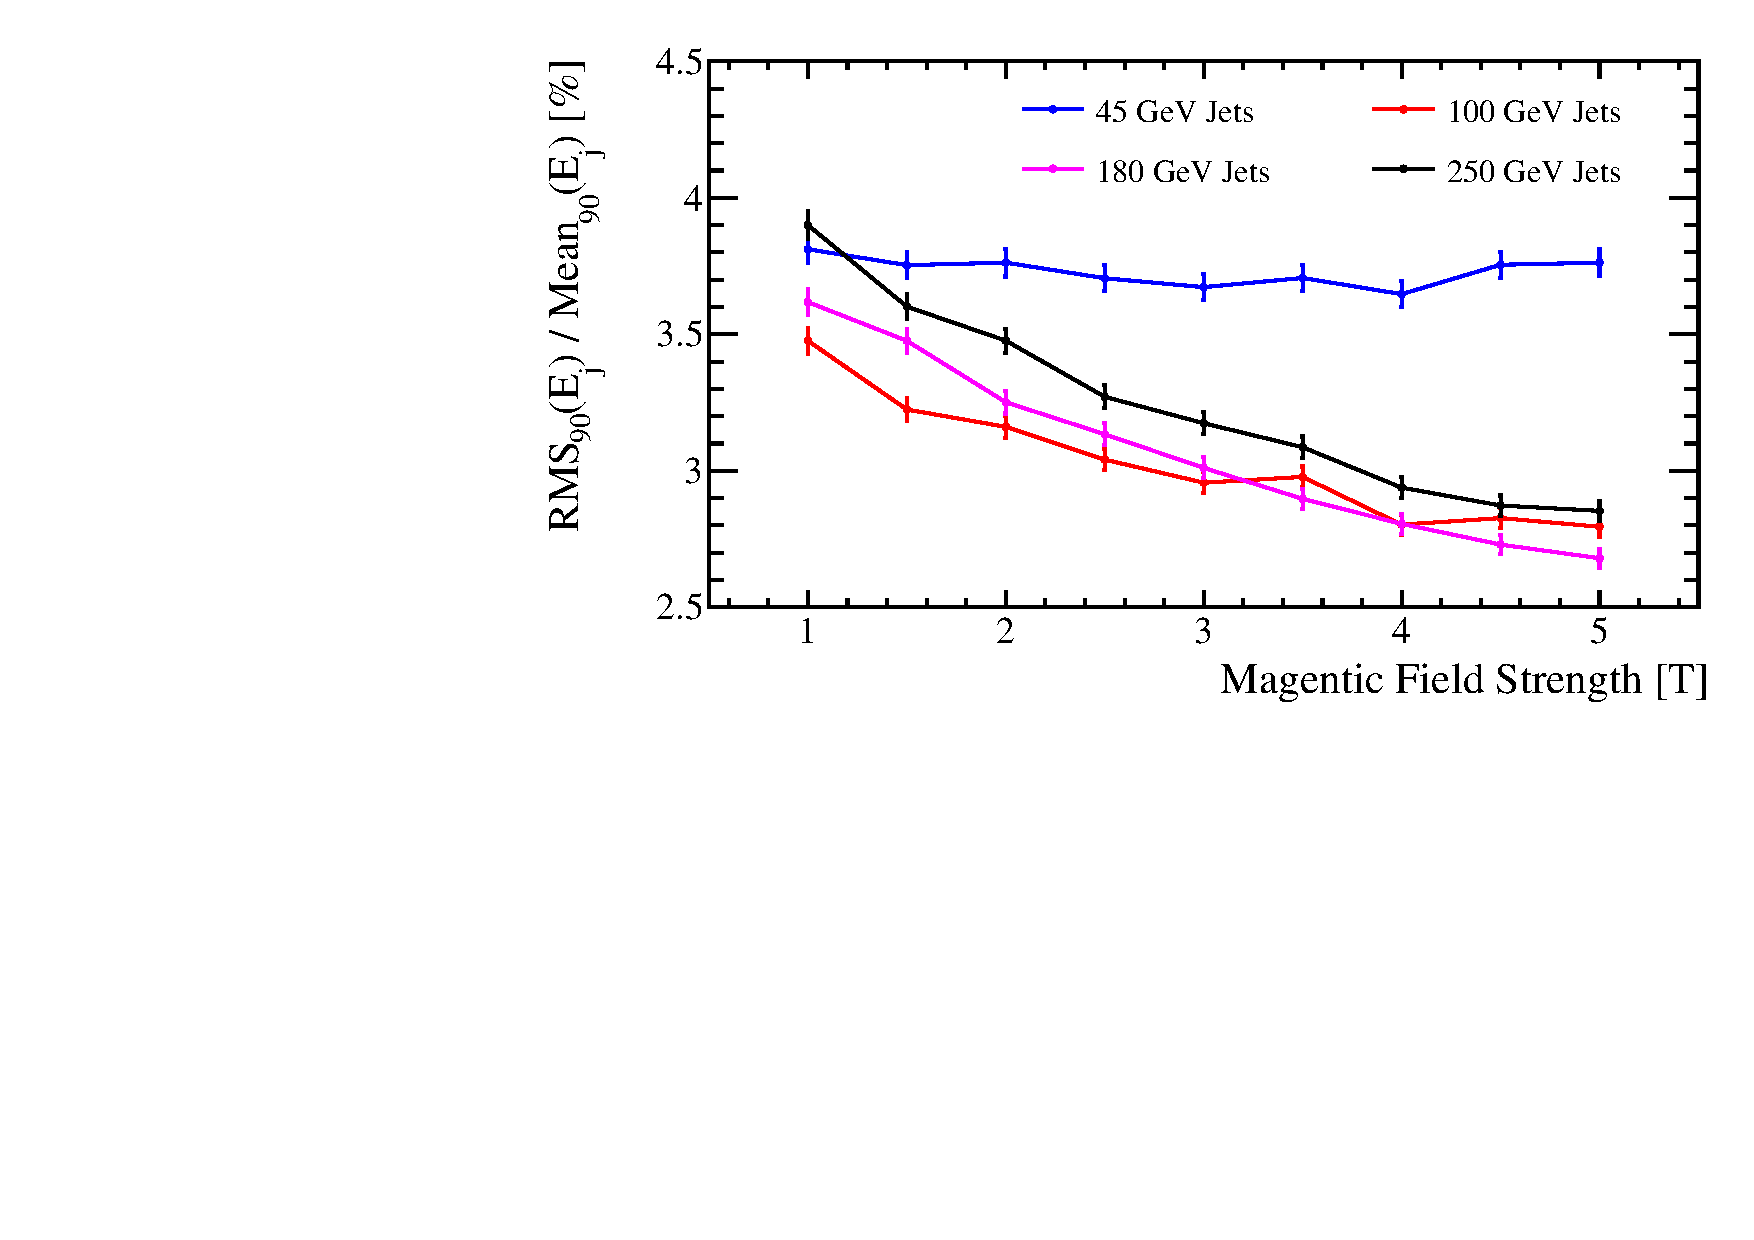
\includegraphics[width=\largefigwidth]{OptimisationStudies/Plots/JER_vs_MagneticField.pdf}
  \caption[Jet energy resolution as a function of magnetic field strength.]{Jet energy resolution is shown for several fixed energy jets as a function of magetic field strength.}
  \label{optstud:fig:bfield}
\end{figure}

\subsection{Inner ECal Radius}
\label{optstud:sec:glob:ecalinnerrad}

\begin{figure}
  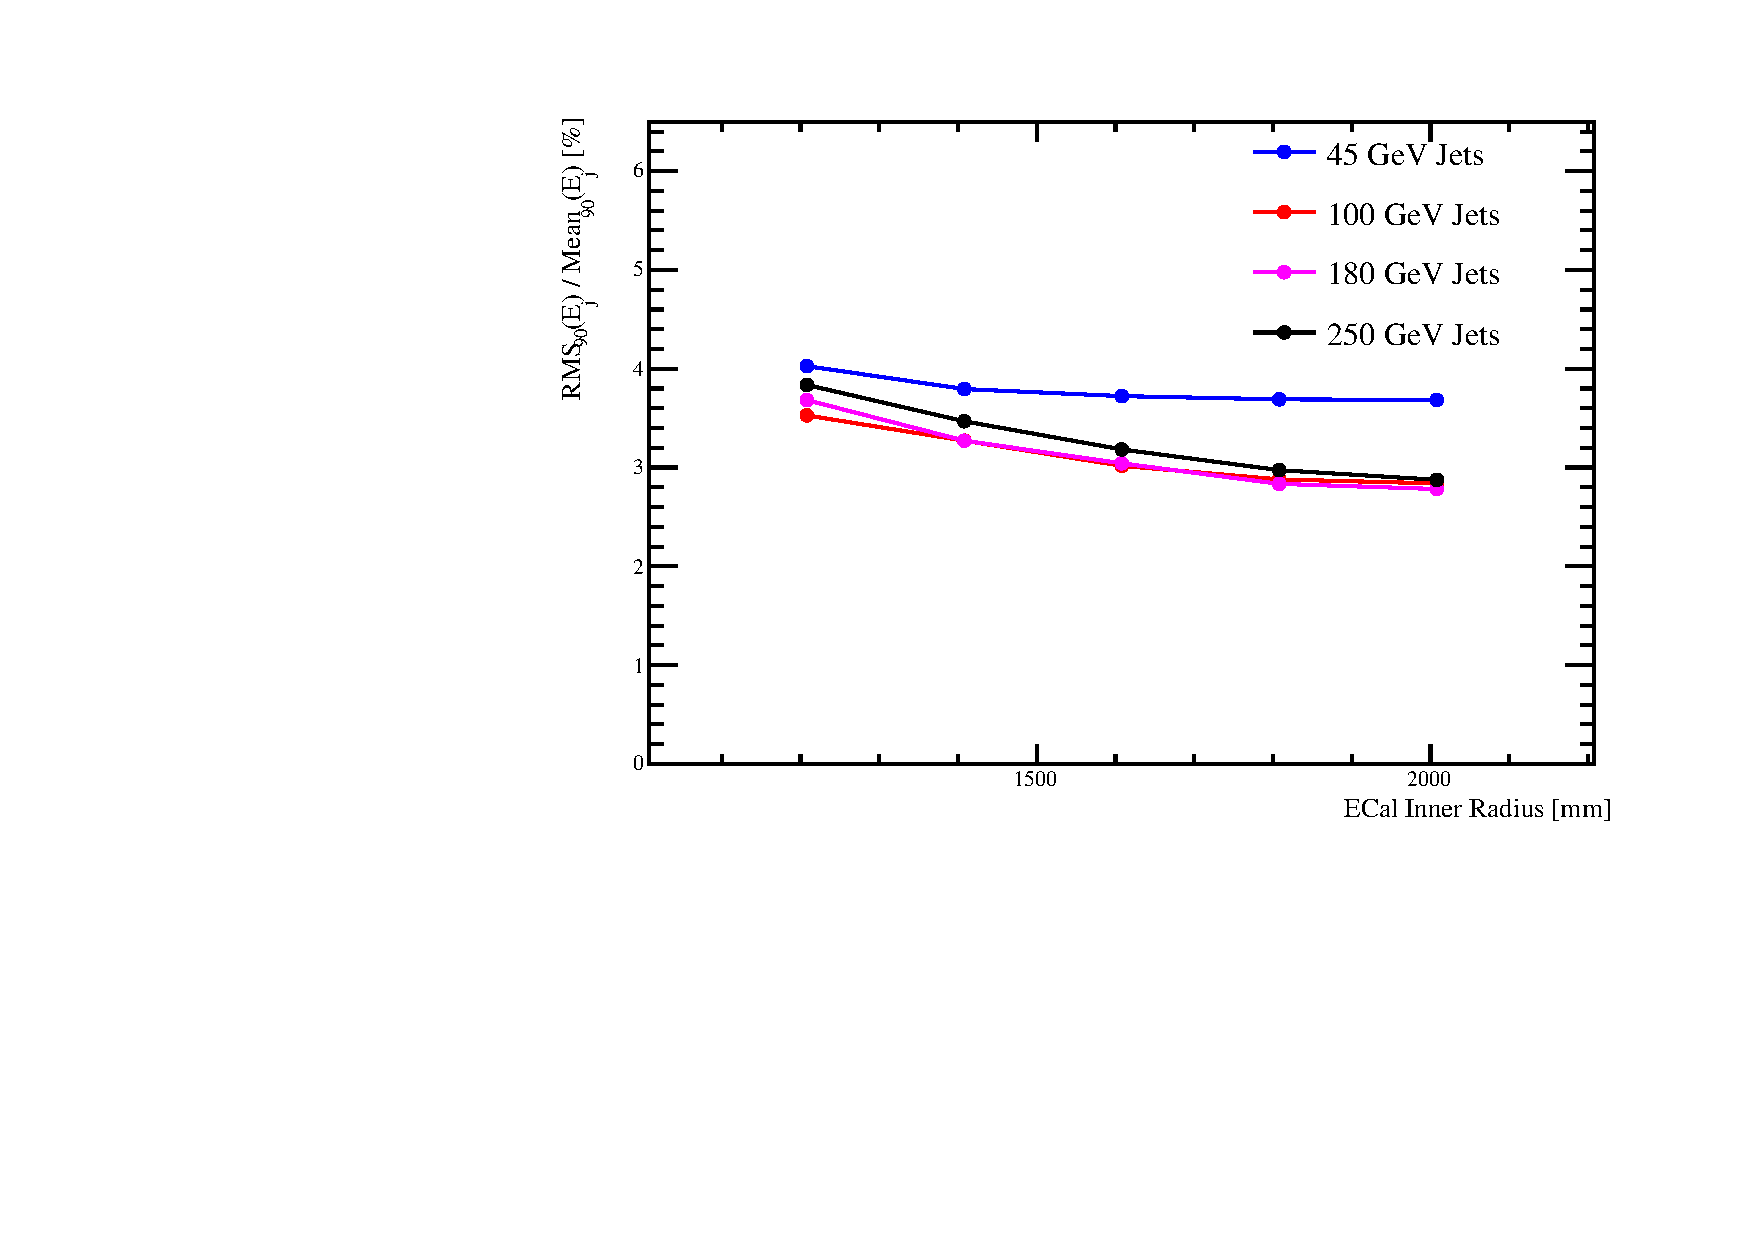
\includegraphics[width=\largefigwidth]{OptimisationStudies/Plots/JER_vs_ECalInnerRadius.pdf}
  \caption[Jet energy resolution as a function of the ECal inner radius.]{Jet energy resolution is shown for several fixed energy jets as a function of the inner ECal radius.}
  \label{optstud:fig:ecalinnerrad}
\end{figure}

\iffalse
ECalCellSizeBoth.pdf                                       JER_vs_ScintillatorECalCellSize.pdf
ECalInnerRadius.pdf                                        JER_vs_ScintillatorECalCellSize_500GeV_DiJet_Breakdown.C
HCalCellSize.pdf                                           JER_vs_ScintillatorECalCellSize_500GeV_DiJet_Breakdown.pdf
HCalNumberIntLenght.pdf                                    JER_vs_ScintillatorECalCellSize_91GeV_DiJet_Breakdown.C
HCalNumberOfLayers.pdf                                     JER_vs_ScintillatorECalCellSize_91GeV_DiJet_Breakdown.pdf
HCalSampFraction.pdf                                       JER_vs_ScintillatorECalNumberofLayers.C
JER_vs_BothECalCellSize.C                                  JER_vs_ScintillatorECalNumberofLayers.pdf
JER_vs_BothECalNumberofLayers.C                            JER_vs_SiliconECalCellSize.C
JER_vs_ECalInnerRadius.C                                   JER_vs_SiliconECalCellSize.pdf
JER_vs_ECalInnerRadius.pdf                                 JER_vs_SiliconECalCellSize_500GeV_DiJet_Breakdown.C
JER_vs_HCalAbsorberMaterial.C                              JER_vs_SiliconECalCellSize_500GeV_DiJet_Breakdown.pdf
JER_vs_HCalAbsorberMaterial.pdf                            JER_vs_SiliconECalCellSize_91GeV_DiJet_Breakdown.C
JER_vs_HCalCellSize.C                                      JER_vs_SiliconECalCellSize_91GeV_DiJet_Breakdown.pdf
JER_vs_HCalCellSize.pdf                                    JER_vs_SiliconECalNumberofLayers.C
JER_vs_HCalCellSize1000000GeVMHHHE.C                       JER_vs_SiliconECalNumberofLayers.pdf
JER_vs_HCalCellSize1000000GeVMHHHE.pdf                     MakePlots.C
JER_vs_HCalCellSize1GeVMHHHE.C                             NumberLayersECalBoth.pdf
JER_vs_HCalCellSize1GeVMHHHE.pdf                           ScECalCells.pdf
JER_vs_MagneticField.pdf                                   ScECalConfusion500GeV.pdf
JER_vs_MagneticFieldStrength.C                             ScECalConfusion91GeV.pdf
JER_vs_MagneticFieldStrength.pdf                           ScECalLayers.pdf
JER_vs_NumberOfLayersInTheHCal.C                           SiECalCells.pdf
JER_vs_NumberOfLayersInTheHCal.pdf                         SiECalConfusion500GeV.pdf
JER_vs_NumberOfNuclearInterationLengthsInTheHCal.C         SiECalConfusion91GeV.pdf
JER_vs_NumberOfNuclearInterationLengthsInTheHCal.pdf       SiECalLayers.pdf
JER_vs_SamplingFractionInTheHCal.C                         SiECalNumberOfLayers.pdf
JER_vs_SamplingFractionInTheHCal.pdf                       SiliconECalCells.pdf
JER_vs_ScintillatorECalCellSize.C
\fi


